\newpage
\stepcounter{handout}
\begin{exercisebox}[adjusted title= Finite state machines]

\begin{minipage}{1.0\linewidth}
\begin{wrapfigure}[9]{r}{0.15\textwidth}
   \vspace{-1em}
   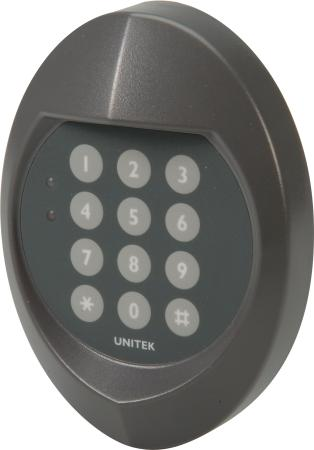
\includegraphics[width=0.15\textwidth]{illustrationer/unitek_kombinationslaas.jpg}
\end{wrapfigure}
 
As the first example of a state machine, we will create one
electronic combination lock, such as those used for access control
doors.

\noindent
Tilstandsdiagram:

\noindent
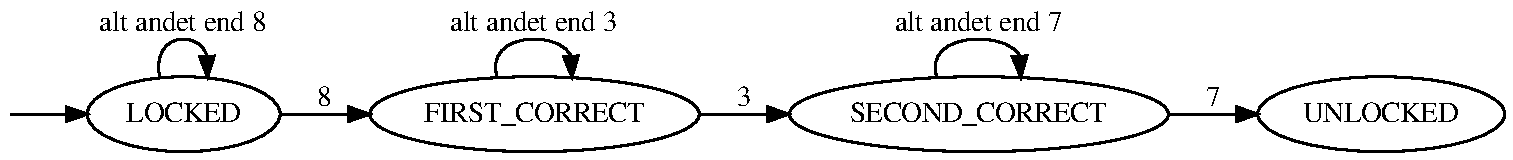
\includegraphics[width=0.85\textwidth]{graphviz/combinationLock_dumb}

%%% FIX!!!!
Download the Processing.py code for the combination lock here:
\mbox{\url{http://kortlink.dk/ufdh}} and copy it into a new Processing project.

\end{minipage}

\begin{itemize}
\item Test the combination lock and watch as the state changes. If you
did not know the ransom (password), how many attempts does it require?
to guess?

\item Change the code so that the default is 524 instead
\item Try changing the code to follow this diagram instead, where incorrect presses reset the state to start:
 
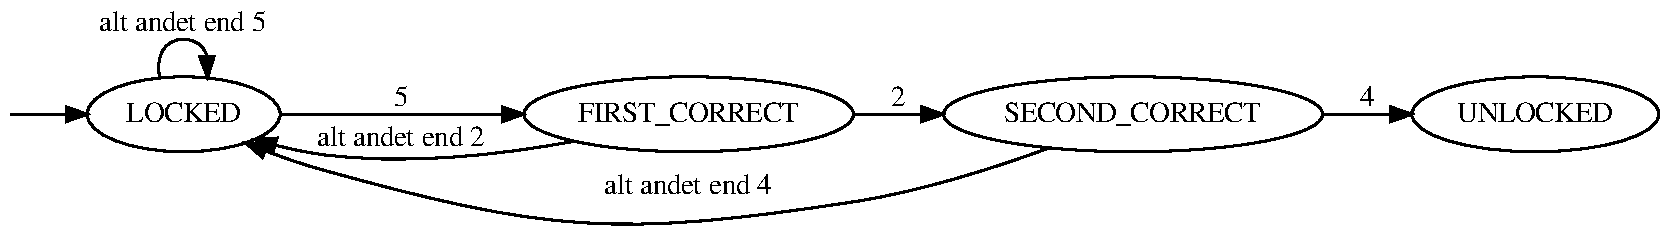
\includegraphics[width=0.85\textwidth]{graphviz/combinationLock_resetting}

\item Draw an extended state diagram of the combination lock with an extra mode, so 4 digits are required. Next, add the extra state in the code.
\end{itemize}
\end{exercisebox}

\begin{exercisebox}[adjusted title= Automatic relock after 2 seconds]

Let's extend the lock so that the door automatically locks again after 2 seconds,
which corresponds to 120 frames:

\noindent
\begin{center}
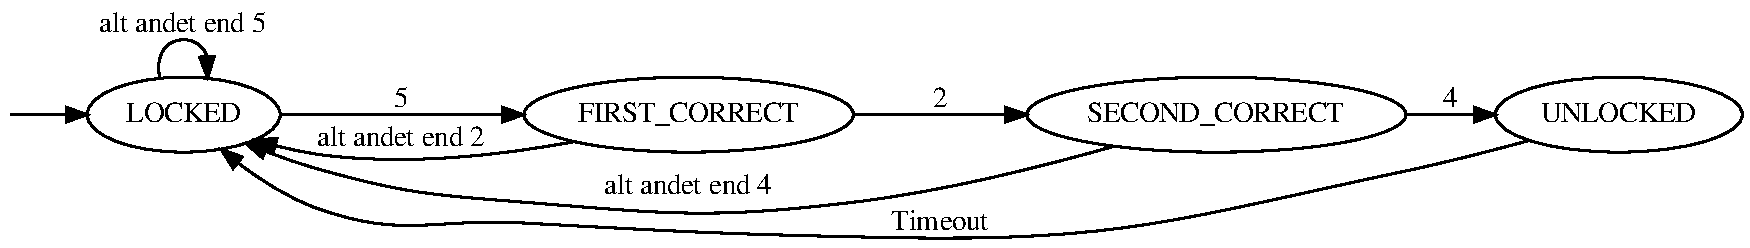
\includegraphics[width=1.0\textwidth]{graphviz/combinationLock_timeout}
\end{center}

\begin{itemize}
\item Create a global variable ``\ttpy{timer}'' and set it to 0
\item Set the \ttpy{timer} variable to 120 as soon as the lock is unlocked, it will
 say when it changes \ttpy{lockState} to \ttpy{"UNLOCKED"}.
\item Count down with the timer in each frame (add the following to the \ttpy{draw} function):


\begin{python}
global timer
if timer > 0:
   timer = timer - 1
\end{python}
\item Når timeren er talt helt ned, skal låsen åbnes. I
 \ttpy{draw}-funktionen skal I nu tjekke om vi er i tilstanden
 \ttpy{"UNLOCKED"} og timeren samtidig er talt ned til 0. Indsæt
 følgende i \ttpy{draw}:
 
\begin{python}
if lockState == "UNLOCKED":
   if timer == 0:
       lockState = "LOCKED"
\end{python}

\end{itemize}
\end{exercisebox}
